\documentclass{beamer}
\usepackage{tikz}
\usepackage{pgfplots}
\usetheme{Warsaw}
\usecolortheme{crane}
\title{Classification of Political News with NLP}
\author{
	Magdaleno, Alejandro\\
	\and
	Lyles-Woods, Quin'darius
}
\institute{Kennesaw State University}
\logo{
\includegraphics[height=1cm]{kennesawlogo}}
\begin{document}
\frame{\titlepage}

\begin{frame}{Outline}
	\tableofcontents
\end{frame}

\section{Proposed Research}
\begin{frame}{Proposed Research}
\begin{itemize}
	\item<1-> The study of an aggregation of news articles. 		\pause
	\item<2-> Using various Natural Language Processing Techniques.     \pause
	\item<3-> Detection of bias with news outlets for the reader.
\end{itemize}
\end{frame}

\section{Goals}
\begin{frame}{Goals}
	\begin{itemize}
		\item<1-> To determine where bodies of text come from algorithmically.
		\item<2-> To have a success rate about 70\% with said goal.
		\item<3-> To understand the success and failures and reaching the goal.
	\end{itemize}
\end{frame}

\section{Relevance}
\begin{frame}{Relevance}
	\begin{itemize}
		\item<1-> Uncovering bias may get us closer to the truth.
		\item<2-> Will be one of the first tools to give a metric to news articles.
		\item<3-> If utilized correctly could be used to save some time when there is more subjective bias than there is fact.
	\end{itemize}
\end{frame}

\section{Data}
\begin{frame}{Data about our Data}
	\begin{itemize}
		\item<1-> Approximately 30,000 articles from CNN and Fox News. \pause
		\item<2-> Each article is self contained within a text file. \pause
		\item<3-> All articles are from the politics section. \pause
		\item<4-> Contains about a year of news articles from both institutions.
	\end{itemize}

	\scalebox{0.6}{
	\begin{tikzpicture}
		\begin{axis}
			\addplot coordinates
			{
				(0,0)
				(1,3)
				(2,130)
				(3,30000)
			};
		\end{axis}
	\end{tikzpicture}
}

\end{frame}
\subsection{Data Source}
\begin{frame}{Data Source}
	The Data was sourced from CNN and Fox News Sites directly.
	There was no data source appropriate for our means so we gathered it ourselves.
	The sites presented their own individual challenges.
\end{frame}
\subsection{Tools}
\begin{frame}{Tools}
	\begin{itemize}
		\item<1->Curl is a tool for transferring data from or to a server.
		\item<2->Grep searches  for  PATTERNS  in  each  FILE. We used it for its ability to search via REGEX expressions.
		\item<3->Pipes are a builtin within most shells allowing for manipulation of text streams.
		\item<4->Cat allows for the catenation of files.
		\item<5->Pup is a tool used for parsing and extracting information from html.
		\item<6->Node is a JavaScript runtime that allows \\for JavaScript to be ran on a server.
	\end{itemize}
\end{frame}

\subsection{Stages}
\begin{frame}{Stages}
	\begin{itemize}
		\item<1-> Constructing a file with all the links to the respective articles.
			\begin{itemize}
				\item ZSH Shell Scripting to algorithmically call websites.
			\end{itemize}
		\item<2-> Downloading all the HTML articles from the links.
			\begin{itemize}
				\item Using the wget (similar to curl) to download each article from text file.
			\end{itemize}
		\item<3-> Parsing the data for only the article bodies.
			\begin{itemize}
				\item Using pup to get the article body and writing the output to a correct file.
			\end{itemize}
		\item<4-> Cleaning up the folder structure.
	\end{itemize}
\end{frame}

\section{Models and Algorithms}
\begin{frame}{Models and Algorithms}
	Tensor Flow is utilized initially to create TF and IDF for the algorithm.
	Then the model takes in the raw text files and puts them together vectorize the text into integer vectors.
	This is utilized with a Sequential Feed-Forward Network to make the base model.
\end{frame}

\subsection{Options to Implement}
\begin{frame}{Options to Implement}
	\begin{itemize}
		\item<1-> TF-IDF
		\item<2-> FastText
		\item<3-> Deep Learning
			\begin{itemize}
				\item Binary
				\item Multiclass
			\end{itemize}
	\end{itemize}
\end{frame}

\subsection{Model Structure}
\begin{frame}{Model Structure}
	\begin{columns}
		\begin{column}{.5\textwidth}
	\begin{itemize}
		\item<1-> Embedding Layers
		\item<2-> Dropout Layer
		\item<3-> Dense Layer
		\item<4-> Global Average
		\item<5-> Dense
		\item<6-> Final Dense
	\end{itemize}
		\end{column}
		\begin{column}{\textwidth}
			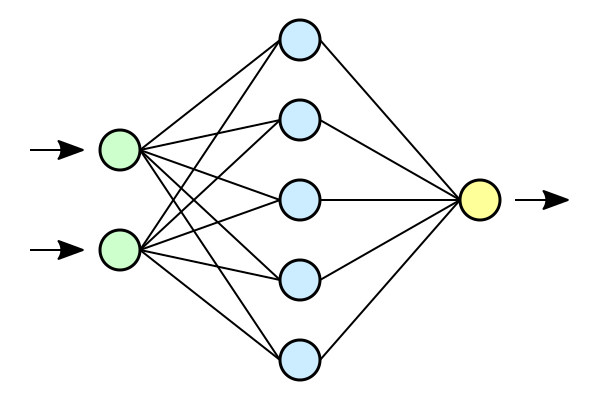
\includegraphics[width=.5\textwidth]{nn}
		\end{column}
	\end{columns}
\end{frame}

\section{Results}
\begin{frame}{Results}
	We ran the model for at most 25 epoch.
	The loss values started very high around 40 percent but as the model ran it went below zero for the loss function and thus the accuracy was around the same and achieving around 99.96 percent accuracy.
\end{frame}

\section{Questions and Answers}
\begin{frame}{Questions and Answers}
	Please ask some questions about anything related to the project.
\end{frame}

\end{document}
